%%%%%%%%%%%%%%%%%%%%%%%%%%%%%%%%%%%%%%%%
%%%%%  xPhO LaTeX Beamer Template  %%%%%
%%%%%  Date: 17/03/2025            %%%%%
%%%%%  Authors:                    %%%%%
%%%%%       Nguyen Thanh Long      %%%%%
%%%%%       Nguyen Le Mai Huong    %%%%%
%%%%%       Nguyen Minh Phuong     %%%%%
%%%%%%%%%%%%%%%%%%%%%%%%%%%%%%%%%%%%%%%%

\documentclass[aspectratio=169, t]{beamer} % Ratio 16:9
\usepackage[T5]{fontenc}
\usepackage{lmodern}
\usepackage{graphicx} 
\usepackage{array}
\usepackage{longtable} % for long table
\usepackage{chngcntr}
\counterwithin{figure}{section}

\renewcommand{\familydefault}{\sfdefault} % Font

\usepackage{caption}
\usepackage{siunitx}

% \definecolor{BlueDefault}{rgb}{0.2,0.2,0.7}
\definecolor{BlueDefault}{RGB}{14,47,95}


% Hide navigation 
\setbeamertemplate{navigation symbols}{}

% Setup background
\newcommand{\normalbackground}{%
    \usebackgroundtemplate{
\includegraphics[width=\paperwidth,height=\paperheight]{Background/Normal_slide_xPhO.pdf}}%
}

\newcommand{\titlebackground}{%
    \usebackgroundtemplate{
\includegraphics[width=\paperwidth,height=\paperheight]{Background/Title_slide_xPhO.pdf}}%
}

% Change the title color to white
\setbeamercolor{frametitle}{fg=white} 

% push the title up by \raisebox
\setbeamertemplate{frametitle}{%
    \vspace{0.3em}
    \hspace{-1em} \insertframetitle
    \vspace{2mm}
}

% Number of slide
\setbeamertemplate{footline}{%
    \hfill
    \insertframenumber/\inserttotalframenumber
    \hspace{7.5mm}
    \vspace{3.5mm}
}

%% Make Table of Contents %%
\AtBeginSection[]{
  \begin{frame}
  \frametitle{Mục lục}
  \vspace{-4mm}
  \tableofcontents[currentsection]
  \end{frame}
}

%% Section numbering %%
\setbeamertemplate{section in toc}[sections numbered]
\setbeamertemplate{subsection in toc}[subsections numbered]


\renewcommand{\figurename}{Hình}
\renewcommand{\tablename}{Bảng}


%%%%% Bibliography %%%%%
\usepackage[backend=biber,style=ieee]{biblatex}
\addbibresource{citation.bib}

\usepackage{url}
\usepackage{hyperref}
\hypersetup{
	colorlinks=true,
	linkcolor=BlueDefault,
	filecolor=BlueDefault,
    citecolor=BlueDefault,
	urlcolor=BlueDefault,
	pdftitle={Overleaf Example},
	pdfpagemode=FullScreen,
}

\begin{document}

\titlebackground

\begin{frame}[noframenumbering]
    \thispagestyle{empty}
    \bfseries
    \begin{flushleft}
        \vfill
        \vspace{5mm}
        \textcolor{BlueDefault}{\huge \bfseries Vector và  \\Nhập môn Đại số tuyến tính} \\
        \vspace{8mm}
        \textcolor{black}{\large \bfseries Người trình bày: Carina }
        \vfill
    \end{flushleft}
\end{frame}

\normalbackground

\section{Nguyên lý tác dụng tối thiểu}

\subsection{Nguyên lý biến phân}

\begin{frame}{Biến phân khác gì với vi phân?}
    \vspace{-4mm}
    \begin{figure}
        \centering
        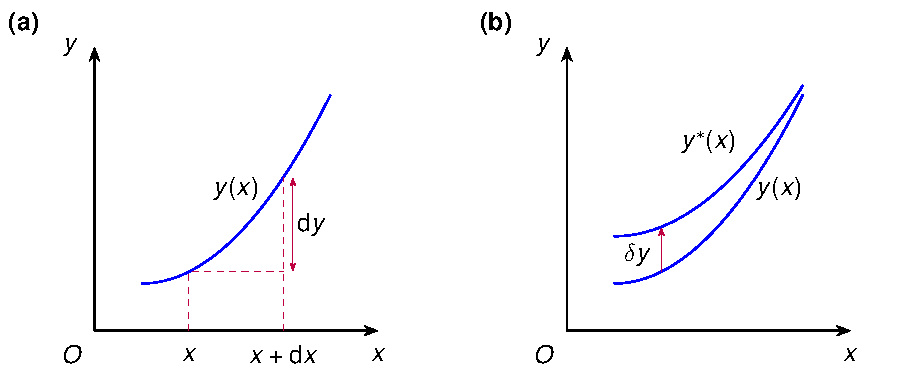
\includegraphics[width=\linewidth]{Figures/Variations.pdf}
        \caption{\textbf{(a)} Phép tính vi phân; \textbf{(b)} Phép tính biến phân. \cite{dao2002cohocgiaitich}}
        \label{fig:Variations}
    \end{figure}
\end{frame}


\subsection{Nguyên lý Maupertuis và nguyên lý Hamilton
về tác dụng tối thiểu}

\begin{frame}{Nguyên lý tác dụng tối thiểu và phương trình Euler}

\begin{columns}
\column{0.6\textwidth}
    \vspace{-3mm}
    \begin{itemize}
        \item Hàm tác dụng \( S \left[\mathbf{q}(t), \dot{\mathbf{q}}(t)\right] \) là tối thiểu.
    \end{itemize}
    \begin{equation}
        S \left[\mathbf{q}(t), \dot{\mathbf{q}}(t)\right] = \int_{t_1}^{t_2} L\left[ \mathbf{q}(t), \dot{\mathbf{q}}(t), t \right] \mathrm{d}t,
    \end{equation}

    \begin{equation} \label{eq:deltaS}
        \delta S = \int_{t_1}^{t_2} \left( \frac{\partial L}{\partial \mathbf{q}} \delta \mathbf{q} + \frac{\partial L}{\partial \dot{\mathbf{q}}} \delta \dot{\mathbf{q}} \right) \mathrm{d}t.
    \end{equation}

    Định lý Leibnitz cho biến phân \(\delta \dot{\mathbf{q}} = \mathrm{d}\left( \delta \mathbf{q} \right) / \mathrm{d}t\)

    \begin{equation}
        \delta S = \int_{t_1}^{t_2} \left( \frac{\partial L}{\partial \mathbf{q}} - \frac{\mathrm{d}}{\mathrm{d}t} \left( \frac{\partial L}{\partial \dot{\mathbf{q}}} \right) \right) \delta \mathbf{q} \mathrm{d}t + \left[ \frac{\partial L}{\partial \dot{\mathbf{q}}} \delta \mathbf{q} \right] \Big|_{t_1}^{t_2}.
    \end{equation}

\column{0.4\textwidth}
    Hàm tác dụng \(S\) đạt cực tiểu khi \(\mathbf{q}(t)\) thỏa mãn phương trình
    \begin{equation}
        \frac{\partial L}{\partial \mathbf{q}} - \frac{\mathrm{d}}{\mathrm{d}t} \left( \frac{\partial L}{\partial \dot{\mathbf{q}}} \right) = 0.
    \end{equation}

    % \begin{itemize}
    %     \item \(L = T - U\) trong cơ học cổ điển.
    %     \item \(L = m c^2 \sqrt{1 - \frac{v^2}{c^2}} \) trong cơ học tương đối tính.
    % \end{itemize}

    \begin{itemize}
        \item Tích phân Euler
    \end{itemize}
    \begin{equation}
        \dfrac{\partial L}{\partial t} + \dfrac{\mathrm{d} }{\mathrm{d} t} \left( \dot{\mathbf{q}} \dfrac{\partial L}{\partial \dot{\mathbf{q}}} - L \right) = 0.
    \end{equation}
    Khi \(\partial L/\partial t = 0\) thì
    \begin{equation}
        H = \dot{\mathbf{q}} \dfrac{\partial L}{\partial \dot{\mathbf{q}}} - L = \text{const}.
    \end{equation}
\end{columns}
    
\end{frame}


\subsection{Các ứng dụng của nguyên lý tác dụng tối thiểu trong vật lý}

\begin{frame}{Catenary - Cực tiểu thế năng trong tĩnh học}
\begin{columns}
\column{0.5\textwidth}
    Thế năng trọng trường của dây xích
    \begin{equation}
        U = \int y \lambda g \sqrt{ y'^2(x) + 1} \mathrm{d} x.
    \end{equation}
    Nên Lagrangian của hệ
    \begin{equation}
        L = \lambda g y \sqrt{ y'^2(x) + 1}
    \end{equation}
    Giải phương trình Euler\footnote{Hoặc tích phân Euler \cite{cline2017variational}.}, ta được
    \begin{equation}
        y = A \cosh \left( \frac{x}{A} \right).
    \end{equation}
    
\column{0.5\textwidth}
    \vspace{-5mm}
    \begin{figure}
        \centering
        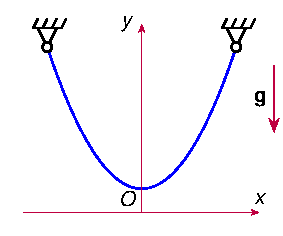
\includegraphics[width=0.9\linewidth]{Figures/Catenary.pdf}
        \caption{Đường Catenary của một dây xích cố định hai đầu đặt trong trọng trường.}
        \label{fig:Catenary}
    \end{figure}
\end{columns}
\end{frame}


\begin{frame}{Nguyên lý Fermat trong quang hình học}

\begin{columns}
\column{0.5\textwidth}
    Thời gian ánh sáng truyền từ \(A\) đến \(B\)
    \begin{equation}
        t = \int_A^B \frac{n}{c} \mathrm{d}s = \frac{1}{c} \int_A^B n(x) \sqrt{1 + y'^2(x)} \mathrm{d}x.
    \end{equation}
    Nên Lagrangian của hệ
    \begin{equation}
        L = n(x) \sqrt{1 + y'^2(x)}.
    \end{equation}
    Giải phương trình Euler, ta được
    \begin{equation}
        n(x) \frac{y'}{\sqrt{1 + y'^2}} = \text{const}.
    \end{equation}
\column{0.5\textwidth}
    \vspace{-9mm}
    \begin{figure}
        \centering
        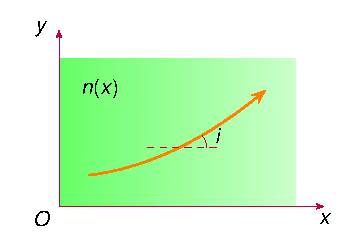
\includegraphics[width=0.9\linewidth]{Figures/Gradient_index.pdf}
        \caption{Ánh sáng truyền trong môi trường có chiết suất biến thiên theo vị trí.}
        \label{fig:Gradient_index}
    \end{figure}
    \vspace{-4mm}
    \begin{itemize}
        \item \(n(x) \sin (i) = \text{const}\) (định luật Snell).
    \end{itemize}
\end{columns}


\end{frame}


\section{Cơ học Lagrange}

\subsection{Nguyên lý D'Alembert về công ảo}

\begin{frame}{Nguyên lý D'Alembert về công ảo}
\vspace{-4mm}
\begin{columns}
\column{0.4\textwidth}
    \begin{itemize}
        \item Nguyên lý công ảo
    \end{itemize}
    \begin{equation}
        \sum_{i} \left( \mathbf{F}_i - \dot{\mathbf{p}}_i \right) \cdot \delta \mathbf{r}_i = 0.
    \end{equation}
    \begin{itemize}
        \item Biến đổi sang tọa độ suy rộng
    \end{itemize}
    \begin{equation}
        \delta \mathbf{r}_i = \sum_{j} \frac{\partial \mathbf{r}_i}{\partial q_j} \delta q_j.
    \end{equation}


    \begin{itemize}
        \item Lực suy rộng
    \end{itemize}
    \begin{equation}
        Q_j = \sum_{i} \mathbf{F}^A_i \cdot \frac{\partial \mathbf{r}_i}{\partial q_j}.
    \end{equation}
    

\column{0.6\textwidth}
    \begin{itemize}
        \item Động lượng
    \end{itemize}
    \begin{equation}
        \dot{\mathbf{p}}_i = \frac{\mathrm{d}}{\mathrm{d} t} \left( \frac{\partial T}{\partial \dot{\mathbf{r}}_i} \right) = \left[ \frac{\mathrm{d}}{\mathrm{d} t} \left( \frac{\partial T}{\partial \dot{q}_j} \right) - \frac{\partial T}{\partial q_j} \right] \frac{\partial \mathbf{r}_i}{\partial q_j}.
    \end{equation}

    \begin{itemize}
        \item Nguyên lý D'Alembert
    \end{itemize}
    \begin{equation}
        \sum_{j} \left[ Q_j - \frac{\mathrm{d}}{\mathrm{d} t} \left( \frac{\partial T}{\partial \dot{q}_j} \right) + \frac{\partial T}{\partial q_j} \right] \delta q_j = 0.
    \end{equation}
    Ta thu được phương trình Euler-Lagrange
    \begin{equation}
        Q_j = \frac{\mathrm{d}}{\mathrm{d} t} \left( \frac{\partial T}{\partial \dot{q}_j} \right) - \frac{\partial T}{\partial q_j}.
    \end{equation}
\end{columns}
\end{frame}

\subsection{Tính toán lực bị động dựa trên phương trình Euler Lagrange}

\begin{frame}{Tính toán lực bị động dựa trên phương trình Euler Lagrange}
\vspace{-4mm}
\begin{itemize}
    \item Tăng thêm tọa độ suy rộng cho cơ hệ thay thế cho liên kết động học? \cite{morin2008introduction}
\end{itemize}
\begin{columns}
\column{0.5\textwidth}
    Lagrangian:
    \begin{equation}
        L = \frac{1}{2} m \left( \dot{r}^2 + \dot{\theta}^2 r^2 \right) -mg r \cos \left( \theta \right).
    \end{equation}

    Phương trình Euler-Lagrange
    \begin{equation}
        N = \frac{\mathrm{d}}{\mathrm{d} t} \left( \frac{\partial L}{\partial \dot{r}} \right) - \frac{\partial L}{\partial r} = m \ddot{r} - m \dot{\theta}^2 r + mg \cos \left( \theta \right).
    \end{equation}

    Tại \(r=R\) không đổi
    \begin{equation}
        N = -m \dot{\theta}^2 R + mg \cos \left( \theta \right).
    \end{equation}
    
\column{0.5\textwidth}
    \begin{figure}
        \centering
        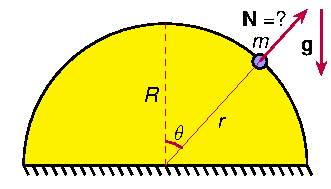
\includegraphics[width=0.9\linewidth]{Figures/Passive_force.pdf}
        \caption{Lực liên kết bị động \(\mathbf{N}\) được tính nhờ khảo sát tọa độ suy rộng \(r\).}
        \label{fig:Passive_force}
    \end{figure}

\end{columns}
\end{frame}

\subsection{Động lượng suy rộng và định lý Noether}

\begin{frame}{Động lượng suy rộng và định lý Noether}
\vspace{-4mm}
\begin{columns}
\column{0.5\textwidth}
    \begin{itemize}
        \item Lagrangian:
    \end{itemize}
    \begin{equation}
        L = \frac{7}{2} m \dot{x}^2 + 3 m \dot{x} \dot{y} + 2 m \dot{y}^2 - mg (x-2y). 
    \end{equation}
    Với phép biến đổi: \(x \to x_0 + \epsilon, y \to y_0 + 2\epsilon\) thì thành phần thế năng \(-mg (x_0 - 2 y_0)\) không phụ thuộc vào \(\epsilon\), nên \(\partial L / \partial \epsilon = 0\)

    \begin{itemize}
        \item Động lượng suy rộng
    \end{itemize}
    \begin{equation}
    \begin{split}
        p_{\epsilon} &= \frac{\partial L}{\partial \dot{x}} \frac{\partial x}{\partial \epsilon} + \frac{\partial L}{\partial \dot{y}} \frac{\partial y}{\partial \epsilon} \\
        &= 17 m \dot{x} + 10 m \dot{y} = \text{const}.
    \end{split}
    \end{equation}

\column{0.5\textwidth}
    \begin{figure}
        \centering
        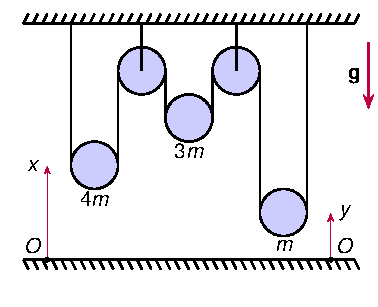
\includegraphics[width=0.9\linewidth]{Figures/Atwoods_machine.pdf}
        \caption{Hệ thống ròng rọc có động lượng suy rộng bảo toàn.}
        \label{fig:Atwoods_machine}
    \end{figure}
    
\end{columns}
\end{frame}

\begin{frame}{Cơ học Lagrange có phải lúc nào cũng là cách tiếp cận tốt nhất?}
\vspace{-2mm}
\begin{itemize}
    \item Lagrangian: \(L = \frac{1}{2} m_1 \dot{q}_1^2 + \frac{1}{2} m_2 \left[ \dot{q}_2^2 + \dot{q}_1^2 - 2 \dot{q}_1 \dot{q}_2 \cos (\theta) \right] - m_2 g q_2 \sin (\theta).\)
\end{itemize}

\begin{columns}
\column{0.5\textwidth}
    Phương trình Euler-Lagrange với \(q_1, q_2\)
    \begin{equation}
    \begin{split}
        & m_1 \ddot{q}_1 + m_2 \left[ \ddot{q}_1 - \ddot{q}_2 \cos (\theta) \right] = 0,\\
        & m_2 \left[ \ddot{q}_2 - \ddot{q}_1 \sin (\theta) \right] = - m_2 g \sin (\theta).
    \end{split}
    \end{equation}

    Hai phương trình trên có thể tìm được từ đâu?
    \begin{itemize}
        \item Bảo toàn động lượng phương nằm ngang.
        \item Định luật II Newton cho khối \(m_2\) chiếu theo phương song song mặt nghiêng.
    \end{itemize}

\column{0.5\textwidth}
    \begin{figure}
        \centering
        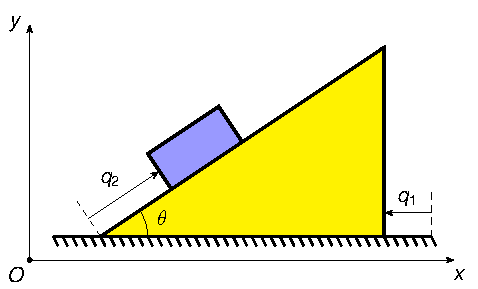
\includegraphics[width=0.9\linewidth]{Figures/Sliding_wedge.pdf}
        \caption{Nêm trượt trên nêm.}
        \label{fig:Sliding_wedge}
    \end{figure}
\end{columns}
\end{frame}



\section{Các nguyên lý cơ học giải tích khác}

\begin{frame}{Có những nền tảng cơ học giải tích nào?}
    \begin{itemize}
        \item Cơ học Lagrange
        \item Cơ học Hamilton
        \item Cơ học Routhian: kết hợp Lagrange và Hamilton.
        \item Nguyên lý Gauss: Hàm cưỡng bức liên kết tối thiểu.
        \item Phương trình Appell: cho cơ hệ phi Holonom.
        \item Koopman–von Neumann: Cơ học lượng tử cổ điển.
    \end{itemize}
\end{frame}

\begin{frame}{Liên kết Holonomic và phi Holonomic}
\vspace{-4mm}
\begin{columns}
\column{0.5\textwidth}
    \begin{itemize}
        \item\textbf{Liên kết Holonomic}
    \end{itemize}
    \begin{equation}
        f \left( \mathbf{q}, t \right) = 0.
    \end{equation}
    \vspace{-9mm}
    \begin{figure}
        \centering
        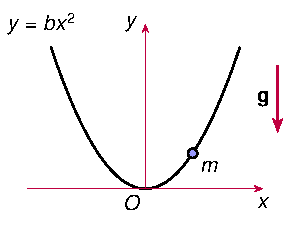
\includegraphics[width=0.8\textwidth]{Figures/Parabol_motion.pdf}
        \vspace{-6mm}
        \caption{Một hạt chuyển động trên bề mặt parabol dưới tác dụng của trọng lực.}
    \end{figure}

\column{0.5\textwidth}
    \begin{itemize}
        \item\textbf{Liên kết phi Holonomic}
    \end{itemize}
    \begin{equation}
        f \left( \mathbf{q}, \dot{\mathbf{q}}, t \right) = 0.
    \end{equation}
    \vspace{-9mm}
    \begin{figure}
        \centering
        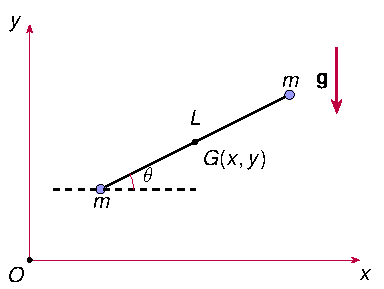
\includegraphics[width=0.8\textwidth]{Figures/NonHolonomic_example.pdf}
        \vspace{-2mm}
        \caption{Một thanh chuyển động dưới tác dụng của trọng trường.}
    \end{figure}
\end{columns}
\end{frame}

\subsection{Cơ học Hamilton}

\begin{frame}{Cơ học Hamilton}

\begin{columns}
\column{0.5\textwidth}
    \begin{itemize}
        \item Biến đổi Legendre: \( H = \sum_{i} p_i \dot{q}_i - L \).
        \item Phương trình Hamilton:
        \vspace{-2mm}
        \begin{align}
            & \dot{q}_i = +\frac{\partial H}{\partial p_i}, \\
            & \dot{p}_i = -\frac{\partial H}{\partial q_i}, \\
            & \frac{\partial H}{\partial t} = - \frac{\partial L}{\partial t}.
        \end{align}
    \end{itemize}
\column{0.5\textwidth}
    \begin{itemize}
        \item Phương trình Hamilton-Jacobi:
        \vspace{-2mm}
        \begin{equation}
            H \left( q_i, \frac{\partial S}{\partial q_i}, t \right) + \frac{\partial S}{\partial t} = 0.
        \end{equation}
        \item Liên hệ trực tiếp với hàm tác dụng \(S\)
        \begin{equation}
            p_i = \frac{\partial S}{\partial q_i}.
        \end{equation}
    \end{itemize}
\end{columns}
\end{frame}

\subsection{Nguyên lý Gauss về liên kết tối thiểu}

\begin{frame}{Nguyên lý Gauss}

\begin{columns}
\column{0.5\textwidth}
    \textbf{Độ cưỡng bức}
    \begin{equation}
        Z = \frac{1}{2} \sum_{i=1}^{N} m_i \left| \mathbf{a}_i - \frac{\mathbf{F}_i}{m_i} \right|^2.
    \end{equation}
    đạt cực tiểu (tức là \(\delta Z = 0, \delta^2 Z > 0\)).

    \textbf{Ví dụ:} \( Z = m \left[ \left( \ddot{x} \right)^2 + \left( \ddot{y} + g \right)^2 \right]\).
    \vspace{-2mm}
    \begin{align}
        & \delta \ddot{y} = 2 b x \delta \ddot{x} \\
        & \delta Z = 2m \left( \ddot{x} \delta \ddot{x} + \left( \ddot{y} + g \right) \delta \ddot{y} \right) = 0 \\
        & \Rightarrow \ddot{x} + 2b x \left( \ddot{y} + g \right) = 0 \\
        & \Rightarrow \left( 1 + 4 b^2 x^2 \right) \ddot{x} + 4 b^2 x \dot{x}^2 + 2 b x g = 0.
    \end{align}

\column{0.5\textwidth}
    \vspace{-6mm}
    \begin{figure}
        \centering
        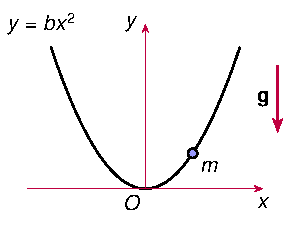
\includegraphics[width=0.9\textwidth]{Figures/Parabol_motion.pdf}
        \vspace{-2mm}
        \caption{Chuyển động của một hạt trên rãnh parabol dưới tác dụng của trọng lực.}
    \end{figure}
\end{columns}

\end{frame}

\subsection{Phương trình Appell cho cơ hệ phi Holonom}

\begin{frame}{Phương trình Appell cho cơ hệ phi Holonom}

\begin{columns}
\column{0.5\textwidth}
    \vspace{-3mm}
    \textbf{Năng lượng gia tốc}
    \begin{equation}
        S = \frac{1}{2} \sum_{i=1}^{N} m_i \left| \ddot{\mathbf{r}}_i \right|^2.
    \end{equation}

    \textbf{Ví dụ:} \( S = m \left[ \ddot{\pi}^2 + L^2 \left( \ddot{\theta}^2 + \dot{\theta}^4 \right) \right] \) 
    với á vận tốc: \( \dot{\pi} = \dot{x}/ \cos ( \theta ) = \dot{y}/ \sin ( \theta )\).

    Biến phân công: \(\delta A = Q_{\pi} \delta \pi + Q_{\theta} \delta \theta\)
    với \( Q_{\pi} = -2 mg \sin ( \theta ), Q_{\theta} = 0\).

    Phương trình Appell
    \vspace{-2mm}
    \begin{align}
        & \frac{\partial S}{\partial \ddot{\pi}} = Q_{\pi}, \quad \frac{\partial S}{\partial \ddot{\theta}} = Q_{\theta} \\
        & \Rightarrow m \ddot{\pi} = -2 mg \sin ( \theta ), \quad m L^2 \ddot{\theta} = 0.
    \end{align}

\column{0.5\textwidth}
    \vspace{-6mm}
    \begin{figure}
        \centering
        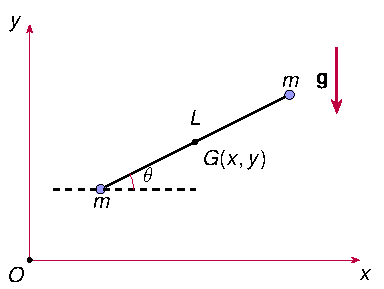
\includegraphics[width=0.9\textwidth]{Figures/NonHolonomic_example.pdf}
        \vspace{-2mm}
        \caption{Một thanh chuyển động dưới tác dụng của trọng trường.}
    \end{figure}
\end{columns}
    
\end{frame}



\begin{frame}[allowframebreaks]{Tài liệu tham khảo}
    \begin{refsection}
        \nocite{morin2008introduction,calculusjame, 3b1b,griffiths2023introduction}
         \printbibliography
    \end{refsection}
\end{frame}

\end{document}